\section{Simulations}
\label{sec:sim}

Our simulations hypothesize two prey species, and five time points.  Of the hierarchy of hypotheses, we simulate data under three null hypotheses: $c, c_s, c_t$.  Sample sizes are randomly chosen from four overlapping levels.  Let ``small'' sample sizes be randomly sampled numbers in $[20,50]$, ``medium'' encompass $[30,75]$, ``large'' $[50,150]$, and ``huge'' $[100,200]$.  Hence, we randomly sample prey and predator gut count observations for each time period from one of the sample size levels, then cycle through all hypotheses.  This is repeated for each level of sample size.  We simulate $500$ replicate datasets for each of the twelve scenarios above for both types of data, fully observed count data, $X_{jst}$, and for non-count data, when we observe only a binary response, $Z_{jst} = 1(X_{jst}>0)$.  A subset of the examples are shown here; the interested reader is referred to the supplementary materials for the complete set of simulation results.

For all simulated data, the true parameter values for the rate at which prey species are encountered in the wild are fixed to be $\gamma_{st} = \pi, \, \forall s,t$. The values of $\lambda_{st}$ are set with respect to each null hypothesis.  For the hypothesis $c_{st} = c$, where predator preferences don't vary by either time or species, we consider $\lambda_{st} = 2\pi, \forall s,t$.  Under the hypothesis $c_s$, the ratio of rates vary by species only, so we put $\lambda_{1t} = \sqrt{2}$ and $\lambda_{2t} = \pi$.  Hence, $c_1 = \sqrt{2}/\pi \approx 0.45$ and $c_2 = 1$.  For the second hypothesis, the ratio of rates vary by time $t$.  Here, we put $\lambda_{st} = t$ for $t \in \{1, \ldots, 5 \}$.  

\begin{figure}
  \centering
  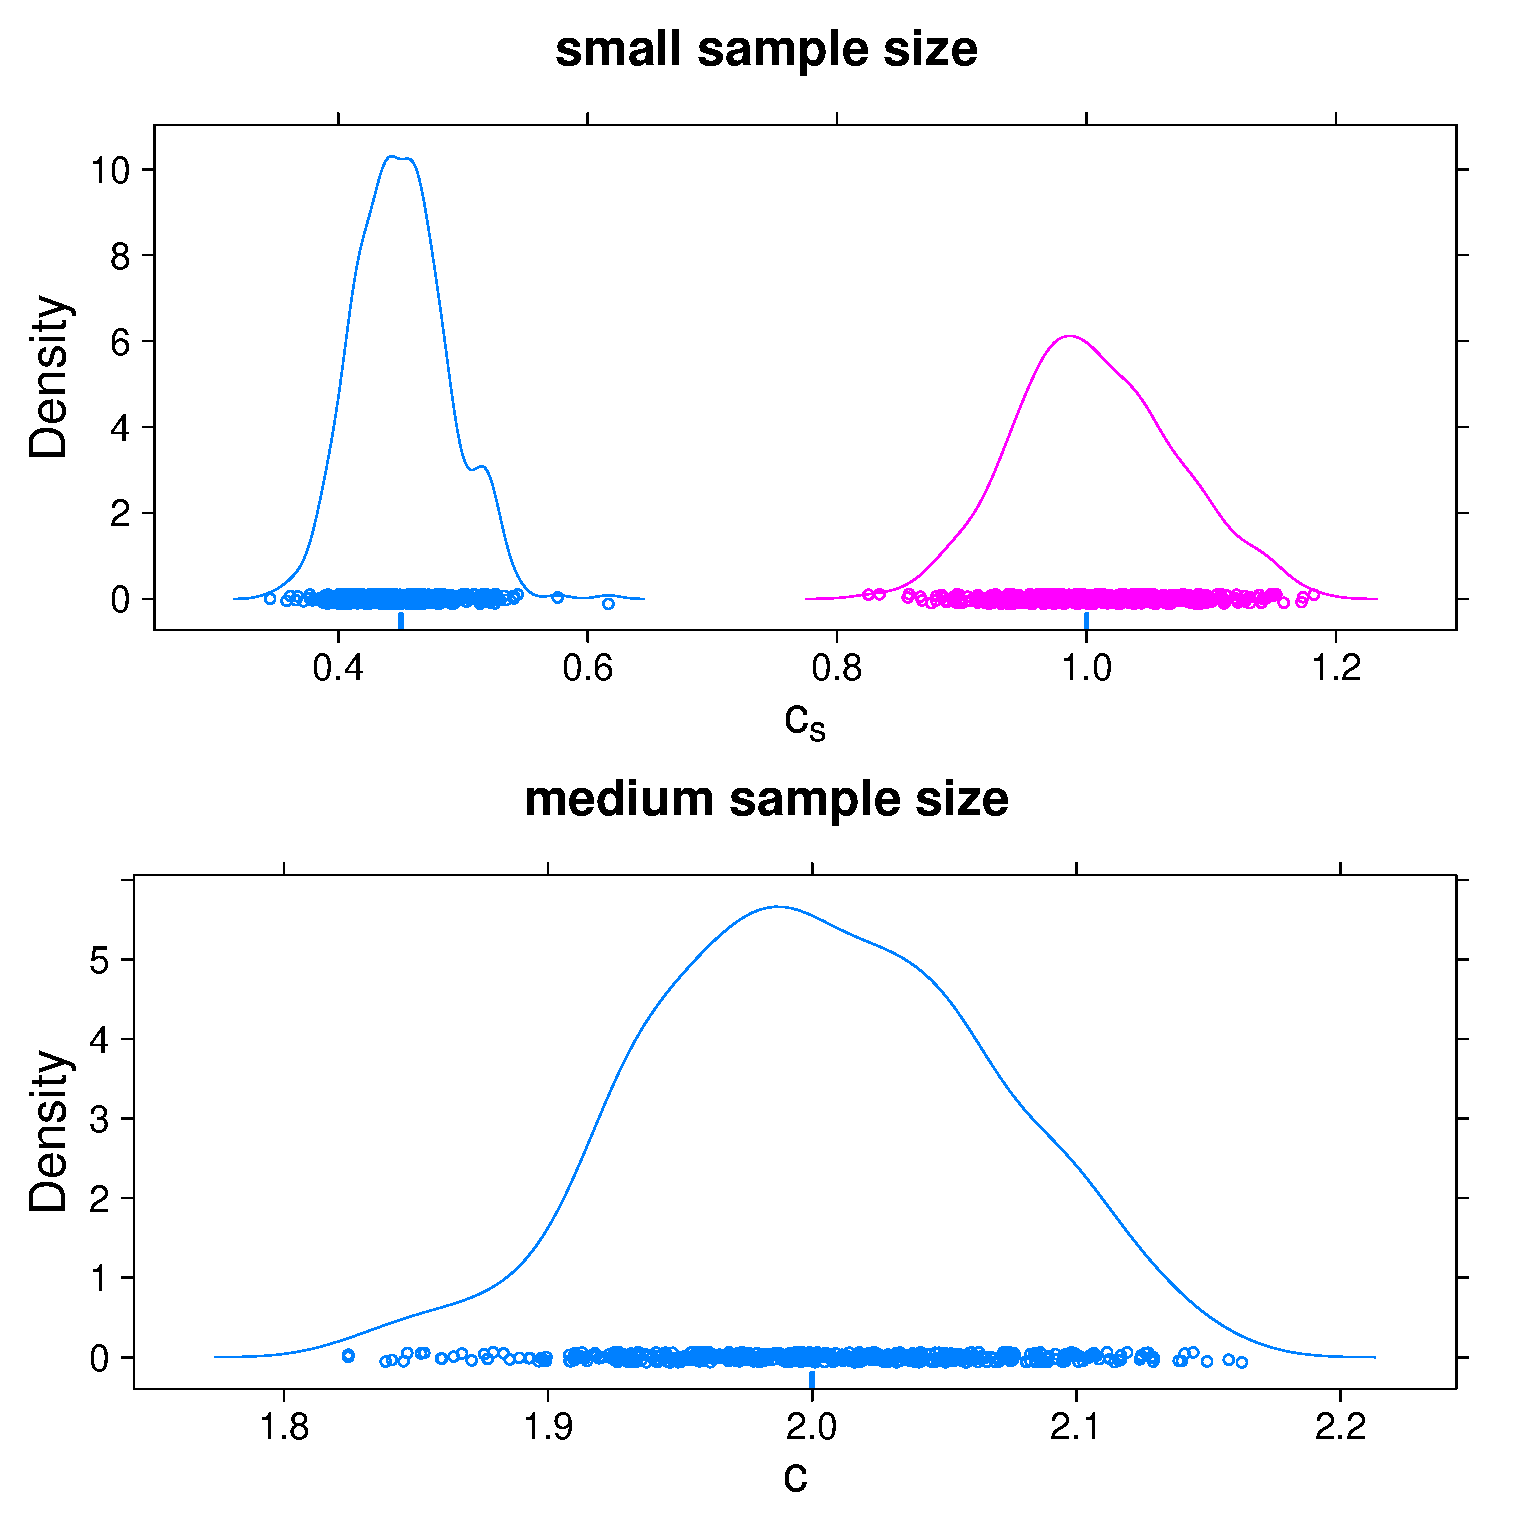
\includegraphics[scale=0.5]{nonem}
  \caption{moar words}
  \label{fig:nonem}
\end{figure}

Figure~\ref{fig:nonem} shows our model fitting to the fully observed count data.  In the first display, the parameters $c_1 \approx 0.4501$ and $c_2 = 1$ are estimated as $\hat{c}_1 = 0.4508$ and $\hat{c}_2 = 1.007$, with standard errors of $\text{se}(\hat{c}_1) = 0.037$ and $\text{se}(\hat{c}_2) = 0.064$.  The second display estimates the parameter $c = 2$ to be $\hat{c} = 2.002$ with standard error $\text{se}(\hat{c}) = 0.065$.  

As noted above we find that the EM algorithm accurately estimates the parameters when values of $\lambda_{st} = c_{st}\gamma_{st}$ are small.  Figure~\ref{fig:em} contains density plots of the EM algorithm's estimates for the hypotheses $c_s,c_t$ for small and huge sample sizes, respectively.  When data are simulated under the null hypothesis $c_s$, we find, even for the small sample size that point estimates are reasonably accurate.  Though, when the values of $\lambda_{st}$ are of sufficient size to make zeros in the simulated data less common, the algorithm occasionally over-estimates the true values.  This effect is easily seen in Figure~\ref{fig:em} for larger values of $c_t$ despite the increased sample size, but it also seen, less dramatically, in the density plot for the hypothesis $c_s$.  The plots of $\gamma_{st}$ under the EM algorithm are not given as we do not consider missing data in the estimation of these parameters. 

\begin{figure}
  \centering
  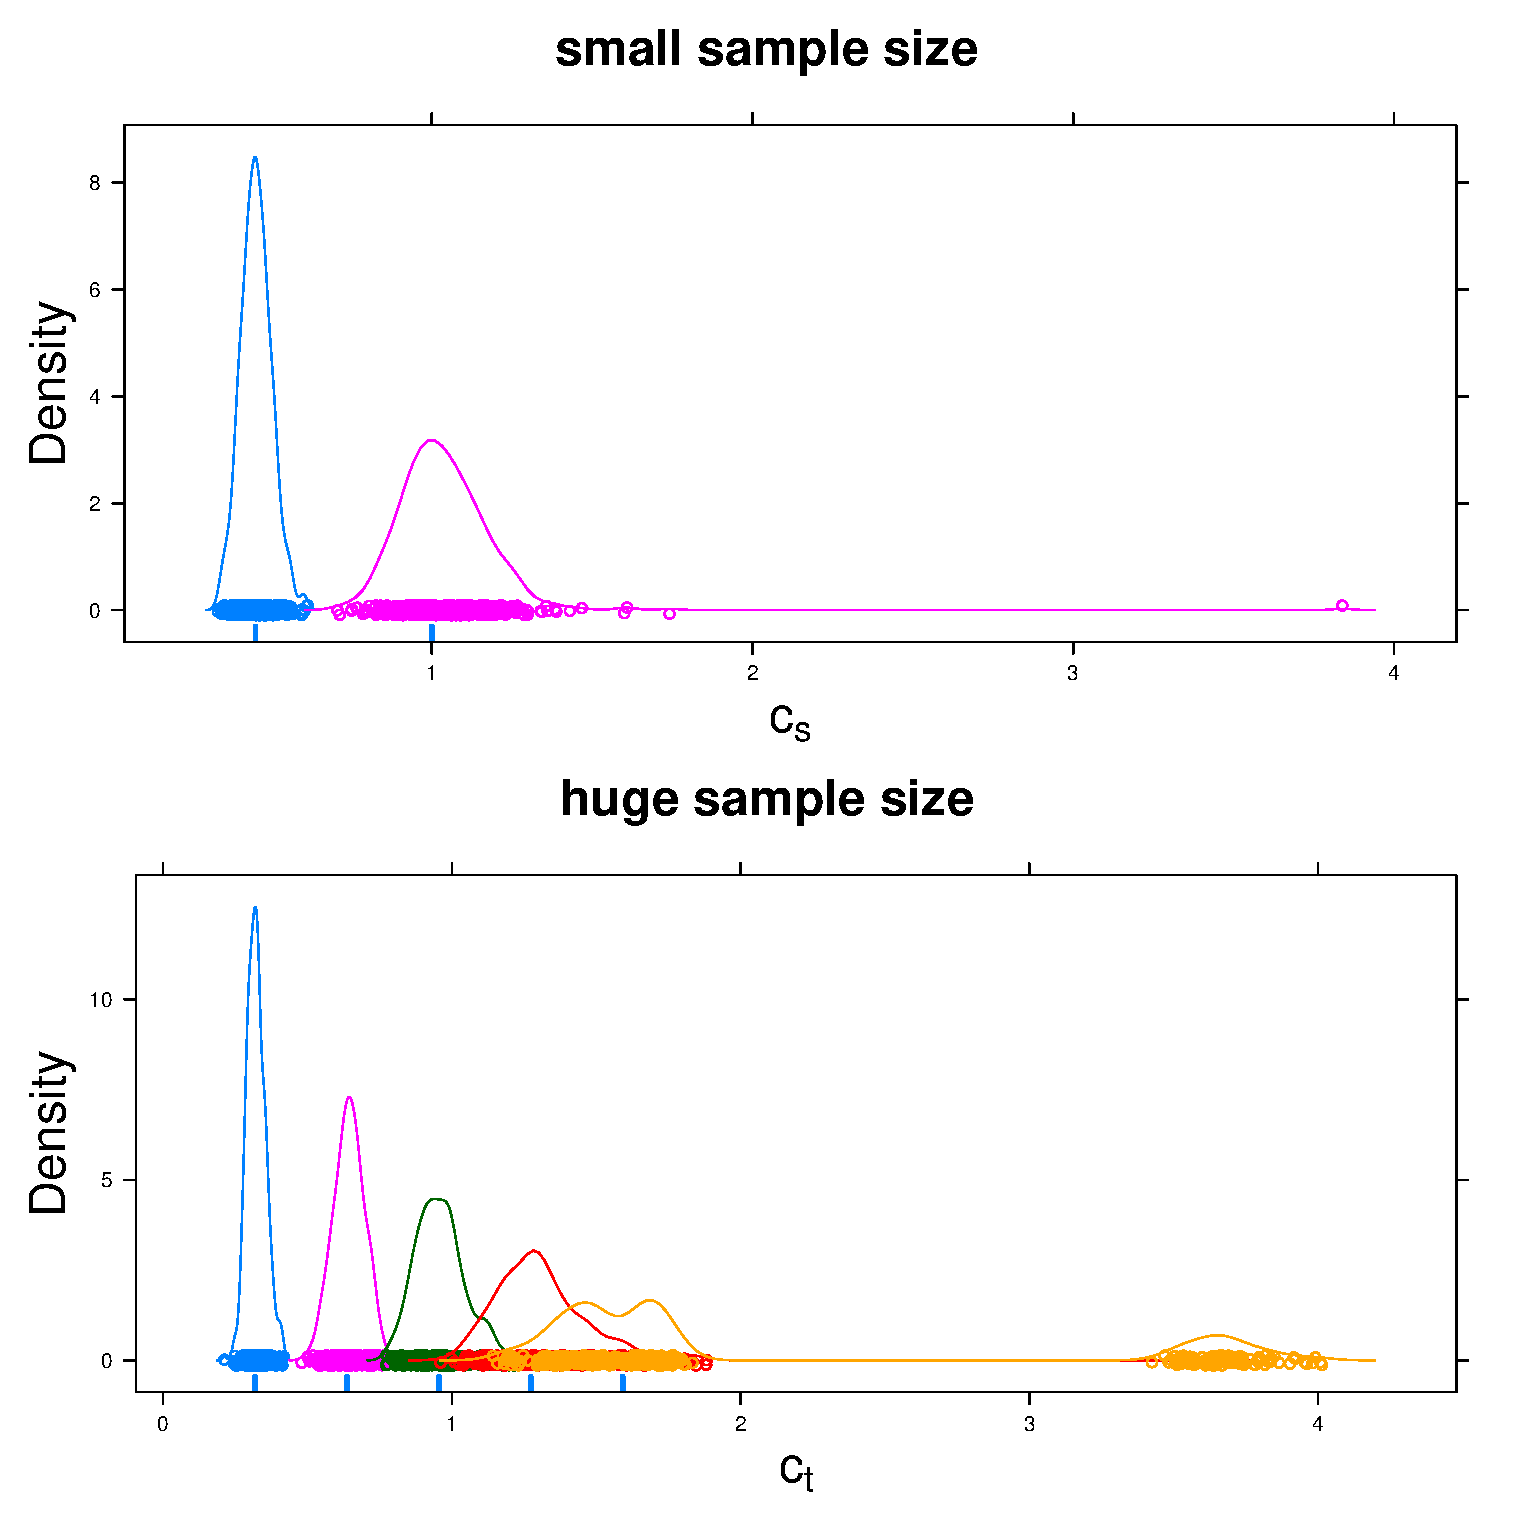
\includegraphics[scale=0.5]{em}
  \caption{Density plots of the EM algorithm's estimates of $c_s$ and $c_t$ with small and huge sample sizes, respectively.  The estimates near $4$ for both of the plots represent samples for which few zeros appeared in the data and the EM algorithm had a particularly difficult time estimating the true parameter value.}
  \label{fig:em}
\end{figure}


Because of the tendency for the EM algorithm to over-estimate some parameter values, bias for non-count data is significantly worse than it is for the count data.  Table~\ref{tab:bias} displays the max absolute bias across all indices $s,t$ of $\lambda_{st}$ for each simulation scenario.  In most cases, these numbers decrease, as expected, as the sample size increases.    

\begin{table}
  \centering
  \begin{tabular}{ll|rrrr}
    & & small & medium & large & huge \\ 
    \hline
    count & $c_t$ & 0.040 & 0.013 & 0.020 & 0.011 \\ 
    & $c_s$ & 0.028 & 0.015 & 0.010 & 0.005 \\ 
    & $c$ & 0.030 & 0.016 & 0.017 & 0.012 \\ 
    non-count & $c_t$ & 4.151 & 3.155 & 0.941 & 1.423 \\ 
    & $c_s$ & 0.138 & 0.096 & 0.044 & 0.032 \\ 
    & $c$ & 2.924 & 2.078 & 0.669 & 0.547 \\ 
  \end{tabular}
  \caption{Max absolute bias of all $\lambda_{st}$ for each simulation scenario.}
  \label{tab:bias}
\end{table}

%%% Local Variables: 
%%% mode: latex
%%% TeX-master: "main"
%%% End: 
